\documentclass[tikz,border=5pt]{standalone}
\usepackage[UTF8]{ctex}
\usepackage{amsmath,amssymb}
\usetikzlibrary{arrows.meta,calc,angles,quotes,positioning,decorations.pathreplacing}
\definecolor{ink}{HTML}{243447}
\definecolor{blue}{HTML}{2765A2}
\definecolor{red}{HTML}{B74739}
\definecolor{green}{HTML}{278365}
\tikzset{line cap=round,line join=round,
body/.style={draw=ink,very thick},
vec/.style={draw=blue,very thick,-{Latex[length=2.3mm]}},
force/.style={draw=red,very thick,-{Latex[length=2.3mm]}},
guide/.style={draw=ink!45,dashed},
dim/.style={draw=ink!75,{Latex[length=1.8mm]}-{Latex[length=1.8mm]}}}
\begin{document}
% question-01: projection of xy plane and concentric rings
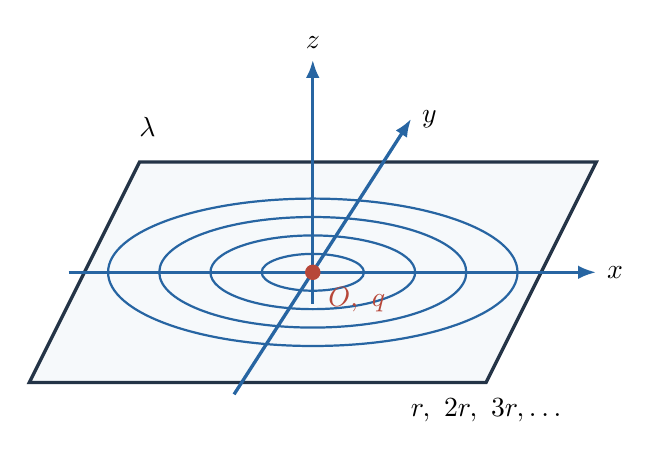
\begin{tikzpicture}
 \fill[blue!4] (-3.6,-1.4)--(2.2,-1.4)--(3.6,1.4)--(-2.2,1.4)--cycle;
 \draw[body] (-3.6,-1.4)--(2.2,-1.4)--(3.6,1.4)--(-2.2,1.4)--cycle;
 \foreach \a in {.65,1.3,1.95,2.6}{\draw[blue,thick] (0,0) ellipse[x radius=\a cm,y radius=.36*\a cm];}
 \draw[vec] (-3.1,0)--(3.6,0) node[right] {$x$};
 \draw[vec] (-1,-1.55)--(1.25,1.95) node[right] {$y$};
 \draw[vec] (0,-.4)--(0,2.7) node[above] {$z$};
 \fill[red] (0,0) circle(2.8pt) node[below right=3pt] {$O,\ q$};
 \node[fill=white,inner sep=2pt] at (2.2,-1.75) {$r,\ 2r,\ 3r,\ldots$};
 \node at (-2.1,1.85) {$\lambda$};
\end{tikzpicture}
% solution-01: single-ring geometry and cone meridian
\begin{tikzpicture}
 \begin{scope}[xshift=-3.8cm]
  \draw[body] (0,0) circle(1.7);
  \draw[vec] (-2,0)--(2.3,0) node[right] {$x$};
  \draw[vec] (0,-1.9)--(0,2.1) node[above] {$y$};
  \coordinate (O) at (0,0); \coordinate (X) at (1.7,0);
  \coordinate (Q) at (50:1.7); \coordinate (P) at (.55,0);
  \draw[guide] (O)--(Q) node[midway,above left] {$a=nr$};
  \draw[red,thick] (P)--(Q) node[midway,right] {$D$};
  \fill[red] (Q) circle(2.7pt) node[above right] {$dq$};
  \fill[blue] (P) circle(2.5pt) node[below] {$P$};
  \draw pic[draw,angle radius=6mm,"$\varphi$"] {angle=X--O--Q};
  \node at (0,-2.4) {单环平面几何};
 \end{scope}
 \begin{scope}[xshift=3.4cm]
  \draw[vec] (-2.1,0)--(2.2,0) node[right] {$\rho$};
  \draw[vec] (0,-1.7)--(0,2.4) node[above] {$z$};
  \fill[blue!6] (0,0)--(1.9,1.45)--(1.9,-1.45)--cycle;
  \draw[body] (-1.9,-1.45)--(1.9,1.45) (-1.9,1.45)--(1.9,-1.45);
  \coordinate (C) at (0,0); \coordinate (R) at (1.9,0);
  \coordinate (S) at (1.35,1.03);
  \draw[red,very thick] (C)--(S) node[midway,above left] {$s$};
  \draw[guide] (S)--(1.35,0) node[midway,right] {$z$};
  \fill[red] (S) circle(2.5pt);
  \draw pic[draw,angle radius=7mm,"$\alpha$"] {angle=R--C--S};
  \node at (0,-2.4) {$\rho=s\cos\alpha,\ z=s\sin\alpha$};
 \end{scope}
\end{tikzpicture}
% question-02: tilted plane in 3D projection
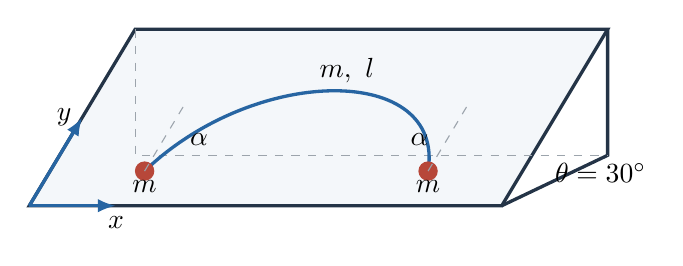
\begin{tikzpicture}[x={(1cm,0cm)},y={(.48cm,.8cm)},z={(0cm,1cm)}]
 \fill[blue!5] (0,0,0)--(6,0,0)--(6,2.8,0)--(0,2.8,0)--cycle;
 \draw[body] (0,0,0)--(6,0,0)--(6,2.8,0)--(0,2.8,0)--cycle;
 \draw[body] (6,0,0)--(6,2.8,-1.6)--(6,2.8,0);
 \draw[guide] (0,2.8,0)--(0,2.8,-1.6)--(6,2.8,-1.6);
 \draw[blue,very thick] (1.2,.55,0) .. controls (1.8,2.25,0) and (4.2,2.25,0) .. (4.8,.55,0);
 \foreach \a in {1.2,4.8}{
  \fill[red] (\a,.55,0) circle(3.5pt);
  \draw[guide] (\a,.55,0)--(\a,1.6,0);
 }
 \node[below] at (1.2,.55,0) {$m$};
 \node[below] at (4.8,.55,0) {$m$};
 \node at (3,2.15,0) {$m,\ l$};
 \node at (1.65,1.05,0) {$\alpha$};
 \node at (4.45,1.05,0) {$\alpha$};
 \draw[vec] (0,0,0)--(1.1,0,0) node[below] {$x$};
 \draw[vec] (0,0,0)--(0,1.4,0) node[left] {$y$};
 \node[right] at (6,1.15,-.5) {$\theta=30^\circ$};
\end{tikzpicture}
% solution-02: force admissibility and arc-length coordinate
\begin{tikzpicture}
 \begin{scope}[xshift=-5.3cm,scale=.83]
  \fill[blue!6] plot[domain=0:.22,samples=80]
    ({20*\x},{20*(.5-sqrt(3/16-\x*\x))})--(4.4,3.5)--(0,3.5)--cycle;
  \draw[blue,thick,domain=0:.22,samples=80]
    plot({20*\x},{20*(.5-sqrt(3/16-\x*\x))});
  \draw[vec] (-.3,0)--(5.4,0) node[right] {$H/(mg)$};
  \draw[vec] (0,-.25)--(0,3.9) node[above] {$V/(mg)$};
  \draw[red,dashed] (0,1.49519)--(4.5,1.49519) node[right] {$V_{\max}/(mg)$};
  \coordinate (O) at (0,0); \coordinate (Y) at (0,3);
  \coordinate (P) at (1.6334674,1.4951905);
  \draw[force] (O)--(P);
  \fill[red] (P) circle(2pt) node[below right] {$P$};
  \draw pic[draw,angle radius=6mm,"$\alpha$"] {angle=P--O--Y};
  \node[blue] at (2.8,3.2) {$f=f_{\max}$};
  \node[align=center] at (2.2,-.85) {$H^2+(mg/2-V)^2\leqslant3m^2g^2/16$};
 \end{scope}
 \begin{scope}[xshift=3.7cm]
  \def\cs{2.3164198}
  \pgfmathsetmacro{\YB}{2-\cs*(cosh(1.9/\cs)-1)}
  \draw[vec] (-2.2,0)--(2.5,0) node[right] {$x$};
  \draw[vec] (0,-.4)--(0,2.5) node[above] {$y$};
  \draw[blue,very thick,domain=-1.9:1.9,samples=60] plot(\x,{2-\cs*(cosh(\x/\cs)-1)});
  \fill[red] (0,2) circle(2.5pt) node[above left] {$C$};
  \fill[red] (1.9,\YB) circle(3pt) node[right] {$B$};
  \fill[red] (-1.9,\YB) circle(3pt) node[left] {$A$};
  \draw[dim] (-1.9,-.45)--(1.9,-.45) node[midway,below] {$D$};
  \draw[force] (1.9,\YB)--++(-1.1,0) node[midway,below] {$H$};
  \draw[force] (1.9,\YB)--++(0,1.00688) node[right] {$V$};
  \foreach \a in {-.8,0,.8}{\draw[green,-{Latex[length=2mm]},thick] (\a,{2-\cs*(cosh(\a/\cs)-1)})--++(0,.65);}
  \node[green] at (1.45,2.65) {$w\,ds$};
  \node at (.75,2.13) {$s$};
  \node at (0,-1.15) {由拱顶量取弧长 $s$};
 \end{scope}
\end{tikzpicture}
% question-03
\begin{tikzpicture}
 \draw[body] (0,0) circle(2);
 \foreach \a/\n/\m in {210/A/m,330/B/2m,90/C/3m}{
  \draw[guide] (0,0)--(\a:2);
  \fill[red] (\a:2) circle(4pt) node[shift={(\a:.45)}] {$\n\ (\m)$};
 }
 \fill[ink] (0,0) circle(2pt) node[below] {$O$};
 \draw[vec] (0,2)--(1.65,2) node[midway,above] {$v_0$};
 \node at (-.9,.55) {$R$};
 \node at (0,-2.7) {水平面内，三个小环相隔 $120^\circ$};
\end{tikzpicture}
% solution-03
\begin{tikzpicture}
 \draw[body] (0,0) circle(2);
 \draw[vec] (-2.5,0)--(3.0,0) node[right] {$x$};
 \draw[vec] (0,-2.5)--(0,3) node[above] {$y$};
 \foreach \a/\n in {210/A,330/B,90/C}{
  \draw[guide] (0,0)--(\a:2);
  \fill[ink] (\a:2) circle(3pt);
 }
 \draw[force] (210:2)--(210:.55) node[midway,left] {$\mathbf a_A$};
 \draw[force] (330:2)--(330:1.15) node[midway,right] {$\mathbf a_B$};
 \node[left=5pt] at (90:2) {$C$};
 \node[below left] at (210:2) {$A$};
 \node[below right] at (330:2) {$B$};
 \draw[force] (90:2)--(90:1.4) node[left=3pt] {$\mathbf a_C$};
 \draw[vec] (0,0)--(.35,1.8) node[above right] {$\mathbf a_O$};
 \node[align=left,anchor=west] at (3.4,1.3)
 {$\mathbf a_O=(a_x,a_y)$\\[4pt]$a_y/2+\sqrt3a_x/2=a_A$\\[4pt]$a_y/2-\sqrt3a_x/2=a_B$\\[4pt]$a_C+a_y=v_0^2/R$};
 \node[align=center] at (0,-3) {红色箭头沿各小环受力方向；蓝色箭头为圆心加速度};
\end{tikzpicture}
% question-04
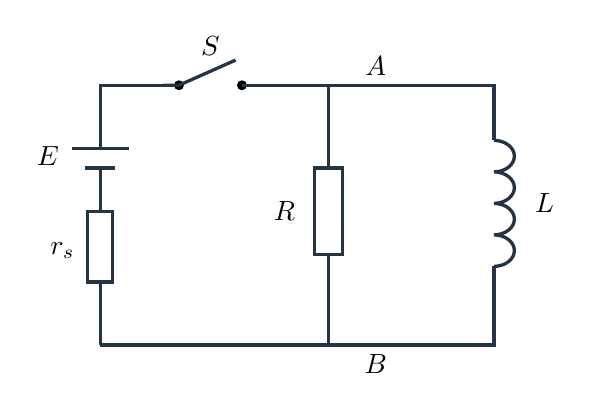
\begin{tikzpicture}
 \draw[body] (0,0)--(5,0)--(5,1);
 \draw[body] (0,0)--(0,.8) (0,1.7)--(0,2.25) (0,2.5)--(0,3.3)--(.8,3.3);
 \draw[body] (-.36,2.5)--(.36,2.5) (-.19,2.25)--(.19,2.25);
 \node[left] at (-.4,2.4) {$E$};
 \draw[body,fill=white] (-.16,.8) rectangle(.16,1.7);
 \node[left] at (-.2,1.2) {$r_s$};
 \fill (1,3.3) circle(1.8pt); \fill (1.8,3.3) circle(1.8pt);
 \draw[body] (.8,3.3)--(1,3.3)--(1.72,3.62);
 \draw[body] (1.8,3.3)--(5,3.3)--(5,2.6);
 \node[above] at (1.4,3.55) {$S$};
 \draw[body] (2.9,3.3)--(2.9,2.25) (2.9,1.15)--(2.9,0);
 \draw[body,fill=white] (2.72,1.15) rectangle(3.08,2.25);
 \node[left] at (2.6,1.7) {$R$};
 \draw[body] (5,2.6) arc[start angle=90,end angle=-90,x radius=.26,y radius=.20]
 arc[start angle=90,end angle=-90,x radius=.26,y radius=.20]
 arc[start angle=90,end angle=-90,x radius=.26,y radius=.20]
 arc[start angle=90,end angle=-90,x radius=.26,y radius=.20];
 \node[right] at (5.4,1.8) {$L$};
 \node[above] at (3.5,3.3) {$A$}; \node[below] at (3.5,0) {$B$};
\end{tikzpicture}
% solution-04
\begin{tikzpicture}
 \foreach \shift/\label/\sgn in {0/闭合阶段/1,5.6/断开阶段/-1}{
  \begin{scope}[xshift=\shift cm]
   \draw[body] (3,.6)--(3,0)--(0,0)--(0,2.8)--(3,2.8)--(3,2.2);
   \draw[body,fill=white] (-.18,.8) rectangle(.18,2);
   \node[left] at (-.22,1.4) {$R$};
   \draw[body] (3,2.2)
    arc[start angle=90,end angle=-90,x radius=.23,y radius=.2]
    arc[start angle=90,end angle=-90,x radius=.23,y radius=.2]
    arc[start angle=90,end angle=-90,x radius=.23,y radius=.2]
    arc[start angle=90,end angle=-90,x radius=.23,y radius=.2];
   \node[right] at (3.3,1.4) {$L$};
   \draw[force] (2.55,2.2)--(2.55,.55) node[midway,left] {$i_L$};
   \ifnum\sgn=1
    \draw[vec] (.55,2.2)--(.55,.55) node[midway,right] {$i_R$};
    \draw[vec] (-1.25,2.8)--(0,2.8) node[midway,above] {$i_s$};
    \node at (1.5,-.75) {$Rq_1=LI_0$};
   \else
    \draw[vec] (.55,.55)--(.55,2.2) node[midway,right] {$|i_R|$};
    \node at (1.5,-.75) {$Rq_{2,\mathrm{alg}}=-LI_0$};
   \fi
   \node at (1.5,3.35) {\label};
  \end{scope}
 }
\end{tikzpicture}
% question-05
\begin{tikzpicture}
 \foreach \shift/\mode in {0/0,5.6/1}{
  \begin{scope}[xshift=\shift cm]
   \fill[blue!5] (-1.4,0) arc[start angle=180,end angle=360,x radius=1.4,y radius=.45]
    --(1.4,-1.0) arc[start angle=0,end angle=-180,x radius=1.4,y radius=.45]--cycle;
   \draw[body] (0,0) ellipse(1.4 and .45);
   \draw[body] (-1.4,0)--(-1.4,-1) arc[start angle=180,end angle=360,x radius=1.4,y radius=.45]--(1.4,0);
   \draw[body] (0,-1.45)--(0,-2) (0,0)--(0,1.8)--(2.5,1.8);
   \draw[body] (1.4,0)--(2.5,0);
   \foreach \x in {-.9,-.45,.45,.9}{\draw[vec] (\x,.1)--(\x,1.05);}
   \node at (-1.4,1.2) {$\mathbf B$};
   \fill[red] (0,0) circle(2pt) node[below right] {$O$};
   \fill[red] (1.4,0) circle(2pt) node[below right] {$A$};
   \ifnum\mode=0
    \draw[body] (2.5,1.8)--(2.5,1.2) (2.5,.6)--(2.5,0);
    \draw[body,fill=white] (2.5,.9) circle(.3) node {$V$};
    \draw[vec] (-.7,-1.7) arc[start angle=190,end angle=350,x radius=.7,y radius=.2];
    \node at (0,-2.5) {发电测量};
   \else
    \draw[body] (2.5,1.8)--(2.5,1.02) (2.5,.77)--(2.5,0);
    \draw[body] (2.3,1.02)--(2.7,1.02) (2.12,.77)--(2.88,.77);
    \node[right] at (2.9,.85) {$E$};
    \node at (0,-2.5) {电池下端接圆周};
   \fi
  \end{scope}
 }
\end{tikzpicture}
% solution-05
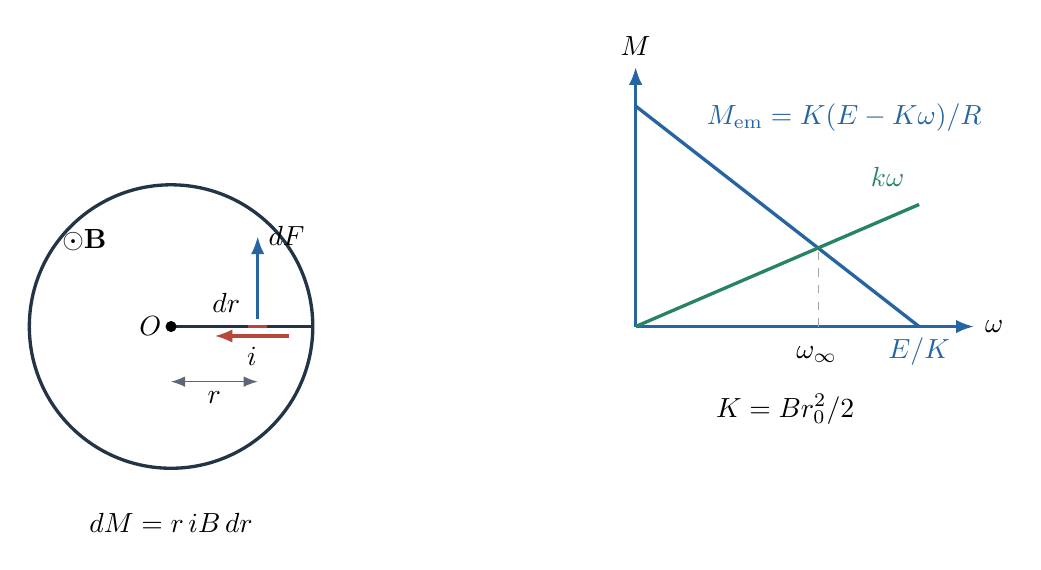
\begin{tikzpicture}
 \begin{scope}[xshift=-3.7cm]
  \draw[body] (0,0) circle(1.8);
  \node at (-1.1,1.1) {$\odot\mathbf B$};
  \draw[body] (0,0)--(1.8,0);
  \draw[force] (1.5,-.12)--(.55,-.12) node[midway,below] {$i$};
  \draw[vec] (1.1,.1)--(1.1,1.15) node[right] {$dF$};
  \draw[dim] (0,-.7)--(1.1,-.7) node[midway,below] {$r$};
  \draw[red,very thick] (.98,0)--(1.22,0);
  \node[above] at (.7,.05) {$dr$};
  \fill (0,0) circle(2pt) node[left] {$O$};
  \node at (0,-2.5) {$dM=r\,iB\,dr$};
 \end{scope}
 \begin{scope}[xshift=2.2cm]
  \draw[vec] (0,0)--(4.3,0) node[right] {$\omega$};
  \draw[vec] (0,0)--(0,3.3) node[above] {$M$};
  \draw[blue,very thick] (0,2.8)--(3.6,0) node[below] {$E/K$};
  \draw[green,very thick] (0,0)--(3.6,1.55);
  \node[blue] at (2.65,2.65) {$M_{\rm em}=K(E-K\omega)/R$};
  \node[green,above] at (3.2,1.65) {$k\omega$};
  \draw[guide] (2.317,0)--(2.317,1.0);
  \node[below] at (2.3,-.13) {$\omega_\infty$};
  \node at (1.9,-1.05) {$K=Br_0^2/2$};
 \end{scope}
\end{tikzpicture}
% question-06
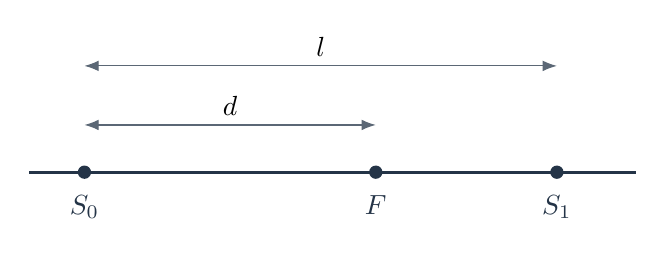
\begin{tikzpicture}
 \draw[body] (-.7,0)--(7,0);
 \foreach \x/\n in {0/S_0,3.7/F,6/S_1}{\fill[ink] (\x,0) circle(2.4pt) node[below=5pt] {$\n$};}
 \draw[dim] (0,.6)--(3.7,.6) node[midway,above] {$d$};
 \draw[dim] (0,1.35)--(6,1.35) node[midway,above] {$l$};
\end{tikzpicture}
% solution-06
\begin{tikzpicture}
 \draw[body] (-5.2,0)--(10.6,0);
 \foreach \x/\n in {0/S_0,3.6/F,6/S_1}{\fill[ink] (\x,0) circle(2.5pt) node[below=3pt] {$\n$};}
 \foreach \x/\n/\lab in {-4.648/O_1/会聚·虚像,2.205/O_2/会聚·实像,4.648/O_3/会聚·实像,9.795/O_4/发散·虚像}{
  \draw[blue,very thick] (\x,-.7)--(\x,.7);
  \node[above] at (\x,.8) {$\n$};
  \node[below,align=center] at (\x,-.85) {\lab};
 }
 \node at (-4.648,1.8) {$-\sqrt{ld}$};
 \node at (2.205,1.8) {$l-\sqrt{l(l-d)}$};
 \node at (4.648,1.8) {$\sqrt{ld}$};
 \node at (9.795,1.8) {$l+\sqrt{l(l-d)}$};
 \begin{scope}[xshift=2.2cm,yshift=-5.6cm]
  \draw[body] (-3,0)--(3,0);
  \draw[body] (-3,0) arc[start angle=180,end angle=0,radius=3];
  \draw[red,very thick] (-1,0)--(-1,2.828);
  \fill[red] (-1,2.828) circle(2.5pt) node[above] {$H$};
  \node[below] at (-3,0) {$A$}; \node[below] at (-1,0) {$C$}; \node[below] at (3,0) {$B$};
  \draw[guide] (-3,0)--(-1,2.828)--(3,0);
  \node[above left] at (-1,1.4) {$\sqrt{a_1b_1}$};
  \draw[dim] (-3,-.65)--(-1,-.65) node[midway,below] {$a_1$};
  \draw[dim] (-1,-.65)--(3,-.65) node[midway,below] {$b_1$};
 \end{scope}
\end{tikzpicture}
% question-07
\begin{tikzpicture}
 \fill[blue!5] (0,0) rectangle(3,2.3);
 \fill[red!4] (3,0) rectangle(6,2.3);
 \draw[body] (0,0) rectangle(6,2.3);
 \draw[body] (2.95,0)--(2.95,.98) (3.05,0)--(3.05,.98)
 (2.95,1.32)--(2.95,2.3) (3.05,1.32)--(3.05,2.3);
 \node[align=center] at (1.4,1.2) {$V_0$\\$2P_0,\ T_0$};
 \node[align=center] at (4.6,1.2) {$V_0$\\$P_0,\ T_0$};
 \draw[vec] (2.45,1.15)--(3.55,1.15);
 \node at (3,-.6) {绝热、刚性容器};
\end{tikzpicture}
% solution-07
\begin{tikzpicture}
 \begin{scope}
  \draw[body] (0,0) rectangle(5.4,2.2);
  \draw[body] (2.7,0)--(2.7,.9) (2.7,1.3)--(2.7,2.2);
  \fill[blue!12] (.03,.03) rectangle(1.45,2.17);
  \draw[blue,dashed,thick] (1.45,0)--(1.45,2.2);
  \node[align=center] at (.72,1.1) {$n_L$\\$V_i$};
  \draw[vec] (1.65,1.1)--(2.45,1.1);
  \node at (2.7,2.75) {追踪最终留在左室的同一团气体};
  \draw[dim] (0,-.45)--(2.7,-.45) node[midway,below] {$V_0$};
 \end{scope}
 \begin{scope}[xshift=7cm]
  \draw[body] (0,0) rectangle(5.4,2.2);
  \draw[body] (2.7,0)--(2.7,.9) (2.7,1.3)--(2.7,2.2);
  \fill[blue!12] (.03,.03) rectangle(2.67,2.17);
  \node[align=center] at (1.35,1.1) {$n_L,\ V_0$\\$P,\ T_L$};
  \node[align=center] at (4.05,1.1) {$n_R,\ V_0$\\$P_R,\ T_R$};
  \node at (2.7,-.8) {$2P_0V_i^\gamma=PV_0^\gamma$};
 \end{scope}
\end{tikzpicture}
% question-08
\begin{tikzpicture}
 \draw[vec] (-.5,-.9)--(8,-.9) node[right] {$x$};
 \draw[body] (0,-.5)--(0,1.2);
 \node[below] at (0,-1.1) {投球、接球位置};
 \foreach \x in {1.1,2.6,4.1}{\draw[body,fill=white] (\x,.4) circle(.12);}
 \draw[vec] (2.6,.4)--(3.6,.4) node[midway,above] {$v_0$};
 \draw[body,fill=blue!6] (6.7,.4) ellipse(.16 and 1.1);
 \draw[vec] (6.4,1.75)--(5.1,1.75) node[midway,above] {$u$};
 \node[below] at (6.7,-1.1) {球拍};
 \draw[dim] (1.1,1.15)--(2.6,1.15) node[midway,above] {$v_0\Delta t$};
 \node at (3.2,-1.8) {$v_0=u=c/2$};
\end{tikzpicture}
% solution-08
\begin{tikzpicture}
 \draw[vec] (0,-.2)--(0,5.6) node[above] {$ct$};
 \draw[vec] (-.2,0)--(4,0) node[right] {$x$};
 \draw[body] (3,0)--(.4,5.2) node[right] {球拍};
 \draw[blue,very thick,-{Latex[length=2.5mm]}] (0,0)--(1.5,3);
 \draw[blue,very thick,-{Latex[length=2.5mm]}] (1.5,3)--(0,4.6154);
 \draw[green,very thick,-{Latex[length=2.5mm]}] (0,1)--(1.25,3.5);
 \draw[green,very thick,-{Latex[length=2.5mm]}] (1.25,3.5)--(0,4.8462);
 \foreach \x/\y/\n in {1.5/3/C_1,1.25/3.5/C_2}{
  \fill[red] (\x,\y) circle(2.6pt) node[right=3pt] {$\n$};
 }
 \draw[dim] (-.7,0)--(-.7,1) node[midway,left] {$c\Delta t$};
 \draw[guide] (1.5,3)--(2.9,3) (1.25,3.5)--(2.9,3.5);
 \draw[dim] (2.8,3)--(2.8,3.5) node[right,midway] {$c\Delta t_c$};
 \draw[guide] (0,4.6154)--(-1.7,4.6154) (0,4.8462)--(-1.7,4.8462);
 \node[anchor=east,align=right] at (-.9,5.1) {$\Delta t_r=3\Delta t/13$};
 \node[anchor=west,align=left] at (4.5,2.7)
 {两次撞拍：$\Delta t_c=\Delta t/2$\\[6pt]
 两次回收：$\Delta t_r=3\Delta t/13$\\[6pt]
 $\Delta p_{\rm ball}=p_{\rm out}-p_{\rm in}$};
\end{tikzpicture}
\end{document}
